\chapter{补充更多细节}
% 对于一些不宜放在正文中的重要支撑材料,可编入毕业论文的附录中。包括某些重要的原始数据、详细数学推导、程序全文及其说明、复杂的图表、设计图纸等一系列需要补充提供的说明材料。如果毕业设计(论文)中引用的实例、数据资料,实验结果等符号较多时,为了节约篇幅,便于读者查阅,可以编写一个符号说明,注明符号代表的意义。附录的篇幅不宜太多,一般不超过正文。

% \section{附录里的图}

% 图 \ref{figA1} 显示……,图 \ref{subfigA1} 表明……。

% \subsection{单张图片}
% \begin{figure}[h]
% 	\centering
% 	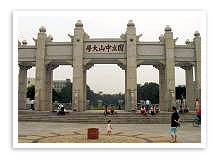
\includegraphics[width=0.8\textwidth]{figure/fig1.png}
% 	\caption{标题} 
% 	\label{figA1}
% \end{figure}

% \subsection{多张子图}
% \begin{figure}[h!] % image examples & compare
% 	\begin{subfigure}{0.55\textwidth}
% 		\centering
% 		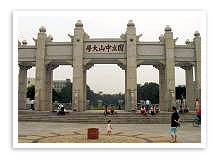
\includegraphics[width=0.5\textwidth]{figure/fig1.png}
% 		\caption{子图1}
% 		\label{subfigA1}
% 	\end{subfigure}
% 	\begin{subfigure}{0.55\textwidth}
% 		\centering
% 		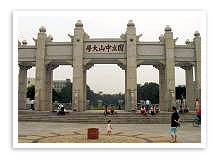
\includegraphics[width=0.5\textwidth]{figure/fig1.png} 
% 		\caption{子图2}
% 		\label{subfigA2}
% 	\end{subfigure}
% 	\begin{subfigure}{0.55\textwidth}
% 		\centering
% 		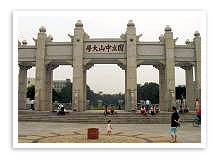
\includegraphics[width=0.5\textwidth]{figure/fig1.png}
% 		\caption{子图3}
% 		\label{subfigA3}
% 	\end{subfigure}
% 	\begin{subfigure}{0.55\textwidth}
% 		\centering
% 		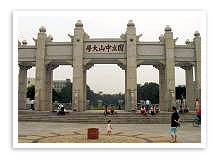
\includegraphics[width=0.5\textwidth]{figure/fig1.png} 
% 		\caption{子图4}
% 		\label{subfigA4}
% 	\end{subfigure}
% 	\caption{多子图}
% 	\label{subfigA}
% \end{figure}




% \section{附录里的表格}
% 表 \ref{tabA1} 表示……。
% \begin{table}[h]
% 	\centering
% 	\caption{国际单位制中具有专门名称的导出单位}		
% 	\label{tabA1}
% 	\begin{tabular}{c|c|c|c}
% 		\toprule[2pt]
% 		量的名称 & 单位名称 & 单位符号 & 其他表示式例\\
% 		\midrule[2pt]
% 		频率	& 赫[兹]	& Hz	&$s^{-1}$ \\
% 		\hline                                        %细横线
% 		力;重力 	& 牛[顿]	& $N$	 & $kg·m/s^2$ \\
% 		\hline                                         %细横线
% 		压力,压强;应力	& 帕[斯卡]	&$Pa$	&$N/m^2$ \\
% 		\bottomrule[2pt]
% 	\end{tabular}
% \end{table}

% \section{附录里的公式}
% \label{sec:formula}
% \begin{equation}
% \label{eqA1}
% \textbf{H} = \begin{bmatrix}
% I*\bm {x}_i \\ \textbf{h}
% \end{bmatrix}
% \end{equation}

% \endinput


\section{NSGA-II 快速非支配排序}
\label{sec:nondominated}

\begin{algorithm}
	% \SetKwFunction{GetLocation}{GetLocation}
	% \SetKwFunction{Partition}{Partition}
	% \SetKwFunction{Sort}{Sort}
	% \SetKwFunction{Int}{Int}
	
	
	% hardBlocks = \{DSP48, BRAM, URAM\}\;
	% \ForEach {hardBlock in hardBlocks}{
	% 	location = \GetLocation{hardBlock, genotype}\;
	% 	\tcp{partition location into columns}
	% 	location\_columns = \Partition{location, distribution}\;
	% 	\ForEach {l\_column in location\_columns} {
	% 		\Sort{l\_column, ascending}\;
	% 		\For{$i\leftarrow 0$ \KwTo l\_column.length} {
	% 			l\_column[i] $\times$= columnSize\;
	% 			l\_column[i] = \Int{l\_column[i]}\;
	% 			need = (l\_column.length-i-1) $\times$ group\_size\;
	% 			avail = columnSize - (l\_column[i] + group\_size)\;
	% 			\If{need $>$ avail}{l\_column[i] -= need - avail\;}
	% 			\ElseIf{l\_column[i] $<$ l\_column[i-1] + group\_size}{
	% 				l\_column[i] = l\_column[i-1] + group\_size\;
	% 			}
	% 		}
			
			
	% 	}
    % }
    
    \ForEach{p $\in$ P}{
        $S_p$ = $\phi$
        $n_p$ = 0
        \ForEach{q $\in$ P}{
            \If{p $\prec$ q \tcp*{If $p$ dominates $q$} }{
                $S_p = S_p \cup$ \{q\} \tcp*{Add $q$ to the set of solutions dominated by $p$}
            }\ElseIf{q $\prec$ p }{
                $ n_p = n_p + 1$ \tcp*{Increase the domination counter of $p$}
            }
        }
        \If{$n_p$=0 \tcp*{$p$ blones to the first front}}{
            $p_{rank} = 1$
            $F_1 = F_1 \cup \{p\}$
        }
    }
    $i=1$ \tcp*{Initialize the front counter}
    \While{$F_i \neq \phi$}{
        $Q = \phi$ \tcp*{ Used to store the members of the next front}
        \ForEach{$p \in F_i$}{
            \ForEach{$q \in S_p$}{
                $n_q = n_q - 1$
                \If{$n_q$ \tcp*{$q$ belongs to the next front}}{
                    $q_{rank} = i + 1$
                    $Q = Q \cup \{q\}$
                }
                $i = i+ 1$
                $F_i = Q$
            }
        }
    }
    

	\caption{Fast-Non-Dominated-Sort(P)}	
	\label{algo:nondominated}
\end{algorithm}

\section{NSGA-II Crowd-Distance 排序}
\label{sec:crowd}

首先定义Crowd-Comparison Operator:

Crowd-Comparison Operator ($\prec_{n}$)在优化的多个进程中促进结果收敛到一个均匀分布的
帕累托前端(Pareto-Front)。假设种群中每个个体$i$有两个属性:
\begin{itemize}
    \item nondomination rank ($i_{rank}$)
    \item crowding distance ($i_{distance}$)
\end{itemize}
我们可以定义Crowd-Comparion Operator $\prec_{n}$:

$$ i \prec_{n} j \ if\  (i_{rank} < j_{rank})$$
$$ or\  ( (i_{rank} = j_{rank}) $$
$$ and\  (i_{distance} > j_{distance}) )$$

也就是说,在两个nondomination rank不同的解中,我们更倾向于rank较低(较好)的一个。
如果rank相同,则说明两个解在同一个帕累托前端内,此时我们选择拥挤度更低的一个。

\begin{algorithm}
	\SetKwFunction{Sort}{Sort}
    
    $l = |I|$ \tcp*{number of solutions in $I$}
    \ForEach{i}{set $I[i]_{distance}=0$ \tcp*{Initialize distance}}
    \ForEach{objective $m$}{
        $I$ = sort($I$, m) \tcp*{sort using each objective value}
        $I[1]_{distance}$ = $I[l]_{distance}$ = $\inf$ \tcp*{so that boundary points are always selected}
        \For{$i = 2$ to $(l-1)$ \tcp*{for all other points}}{
            $I[i]_{distance} = (I[i]_{distance} + I[i+1].m - I[i-1].m) / (f_m^{max} - f_m^{min})$
        }
    }
	
	\caption{Crowd-Distance-Assignment($I$)}	
	\label{algo:crowd-distance-assign}
\end{algorithm}


\begin{algorithm}
    \SetKwFunction{Fast-Non-Dominated-Sort}{Fast-Non-Dominated-Sort}
    \SetKwFunction{Crowding-Distance-Assignment}{Crowding-Distance-Assignment}
    \SetKwFunction{Sort}{Sort}
    \SetKwFunction{make-new-pop}{make-new-pop}

    $R_t = P_t \cup Q_t$ \tcp*{combine parent and offsprint population}

    $F$ = Fast-Non-Dominated-Sort($R_t$) \tcp*{F is all nondominated fronts of $R_t$}

    $P_{t+1} = \phi$ 

    $i = 1$

    \While{$|P_{t+1}| + |F_i| <= N$ \tcp*{until the parent population is filled}}{

        Crowding-Distance-Assignment($F_i$)

        $P_{t+1}  = P_{t+1} \cup F_i$ \tcp*{include $i$th nondominated front in the parent pop}

        $i = i + 1$ \tcp*{check the next front for inclusion}
    }

    Sort($F_i$, $\prec_n$) \tcp*{sort in descending order using $\prec_n$}

    $P_{t+1} = P_{t+1} \cup F_i[1 : (N - |P_{t+1}|)]$ \tcp*{choose the first $ (N - |P_{t+1}|)$ elements of $F_i$}

    $Q_t+1$ = make-new-pop($P_{t+1}$) \tcp*{use selection, crossover, and mutation to create a new poputlation}

    $t = t + 1$ \tcp*{increment the generation counter}

    

    \caption{Crowd-Distance-Sorting}
    \label{algo:crowd-distance-sorting}
\end{algorithm}